\documentclass[compress]{beamer}

\usepackage{beamerthemeWarsaw}
%\usecolortheme{seagull}
\usefonttheme{serif}
\useoutertheme[subsection=false]{smoothbars}
\usetheme{Warsaw}
\setbeamertemplate{itemize item}[triangle]

\usepackage[T1]{fontenc}       
\usepackage[utf8]{inputenc}    % pour les accents (mettre latin1 pour windows au lieu de utf8)
\usepackage[frenchb]{babel}    % le documents est en français
\usepackage{amsmath}           % un packages mathématiques
\usepackage{xcolor}            % pour définir plus de couleurs 
\usepackage{graphicx}          % pour insérer des figures
\usepackage[french]{algorithm2e}
\usepackage{caption}
\usepackage{float}
\usepackage{subfig}

\logo{
\includegraphics[height=5mm]{logo.png}}  

\setbeamertemplate{footline}{
\leavevmode%
\hbox{\hspace*{-0.08cm}
\begin{beamercolorbox}[wd=.3\paperwidth,ht=2.25ex,dp=1ex,center]{author in head/foot}%
	\usebeamerfont{author in foot}\insertshortauthor%~~(\insertshortinstitute)
\end{beamercolorbox}%
\begin{beamercolorbox}[wd=.5\paperwidth,ht=2.25ex,dp=1ex,center]{section in head/foot}%
	\usebeamerfont{section in foot}\insertshorttitle
\end{beamercolorbox}%
\begin{beamercolorbox}[wd=.2\paperwidth,ht=2.25ex,dp=1ex,right]{section in head/foot}%
	\usebeamerfont{section in foot}\insertshortdate{}\hspace*{2em}
	\insertframenumber{} \hspace*{2ex}
\end{beamercolorbox}}%
\vskip0pt%
}
     
\setbeamertemplate{blocks}[rounded][shadow=true]
     
\title[Développement d'un outil de traitement d'images]{Développement d'un outil de traitement d'images par filtrage bilatéral}
\subtitle{Soutenance de PFE}
\author{Natacha Marlio-Marette}
\institute{\textbf{Polytech Tours} \vspace{.10cm} \\ DI5 2014-2015 \vspace{.10cm} \\ encadré par \\ Moncef Hidane}
\date[11/05/15]{11 avril 2015}

\begin{document}

\frame{
	\titlepage
}

\begin{frame}{Plan}
  \begin{columns}[t]
  \begin{column}{5cm}
  \tableofcontents[sections={1-4}]
  \end{column}
  \begin{column}{5cm}
  \tableofcontents[sections={5-8}]
  \end{column}
  \end{columns}
\end{frame}

\section{Introduction}
\begin{frame}
\frametitle{Introduction}
	\begin{block}{Objectifs}
		\begin{itemize}
			\item Création d'une méthode de manipulation de détails d'une image
			\item Réalisation d'une interface graphique
			\item \'Etude sur l'accélération du filtre bilatéral
		\end{itemize}
	\end{block}
\end{frame}

\section{Filtre bilatéral}
\subsection{Definition}
\begin{frame}\frametitle{Filtre bilatéral}
	\begin{definition}
		Lisse une image en préservant les contours
	\end{definition}
\pause
	\begin{block}{Utilisations}
		\begin{itemize}
			\item Débruitage
			\item Outil de gestion de contraste
			\item Fusion d'images
			\item Lissage 3D
			\item Effet cartoon
		\end{itemize}
	
	\end{block}
\end{frame}

\subsection{Formulation}
\begin{frame}\frametitle{Formulation}
	\begin{block}{Filtre gaussien}
		\begin{itemize}
			\item $GC[I]_p = \sum_{q\in S}G_{\sigma}(\parallel p-q \parallel ) I_q  $
		\end{itemize}		
	\end{block}
\pause	
	\begin{block}{Filtre bilatéral}
		\begin{itemize}
			\item $BF[I]_p = \frac{1}{W_p}\sum_{q\in S} G_{\sigma_s}(\parallel p- q \parallel)G_{\sigma_r}(\mid I_p - I_q \mid) I_q$ 
			\item $W_p = \sum_{q\in S} G_{\sigma_s}(\parallel p- q \parallel)G_{\sigma_r}(\mid I_p - I_q \mid)$
		\end{itemize}
	\end{block}	
\pause	
	\begin{block}{Différences}
		\begin{itemize}
			\item Prise en compte de la valeur des pixels
			\item Image moins "floue"
		\end{itemize}
	\end{block}
	
\end{frame}

\begin{frame}\frametitle{Exemples}
	\begin{figure}
		\centering
		\subfloat[Image originale]{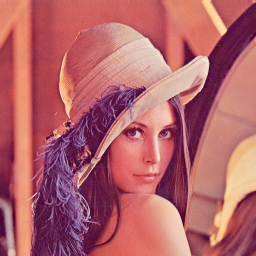
\includegraphics[scale=0.4]{images/lena.png} }
        ~
        % sigma = 3
        \subfloat[Filtre gaussien]{ 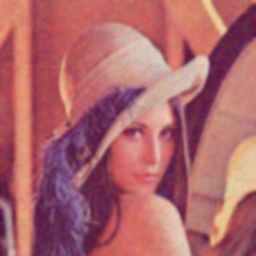
\includegraphics[scale=0.4]{images/lenaGauss.png}}
        ~
        % sigmaS =15 sigmaR = 15
        \subfloat[Filtre bilatéral]{\label{subfig:FBbruitLena} 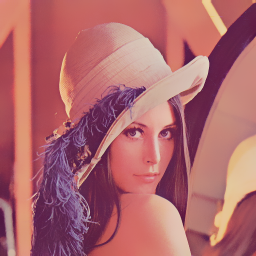
\includegraphics[scale=0.4]{images/lenaFB.png}}
	\end{figure}
\end{frame}

\subsection{Implémentation}
\begin{frame}\frametitle{Algorithme}
\begin{algorithm}[H] \index{Filtre bilatéral}
	\DontPrintSemicolon
%	\Entree{Image $I$}
%	\Sortie{Image filtrée $BF[I]$}
	\BlankLine
	\Pour{$p \in I$ }{
		\tcp{Initialisation}
		$BF[I]_p = 0$ \;
		$W_p = 0$ \;
		\Pour{$q \in S$}{
			$w = G_{\sigma_s}(\parallel p-q \parallel)G_{\sigma_r}(\mid I_p - Iq \mid) $ \;
			$BF[I]_p += wI_q $ \;
			$ W_p += w$ \;
		}
		\tcp{Normalisation}
		$BF[I]_p = BF[I]_p / W_p $  
	}
%\caption{Algorithme général du filtre bilatéral}
\end{algorithm}

\end{frame}

\begin{frame}\frametitle{Luminance}
	\begin{definition}
		\begin{itemize}
			\item Sensation visuelle de luminosité d'une image
			\item Grandeur photométrique qui est dépendante de l'\oe il humain
			\item Différents espaces colorimétriques (CIE XYZ, xyY ou YCbCr)
			\item Y représente la luminance
		\end{itemize}
	\end{definition}
\pause	
	\begin{block}{Algorithme}
		\begin{itemize}
			\item Passage par la luminance
			\item Application du filtre bilatéral sur la composante Y
			\item Retour en RGB
		\end{itemize}
	
	\end{block}
\end{frame}




\section{Validation}
\subsection{Mise en place}
\begin{frame}\frametitle{Mise en place}
	\begin{block}{Méthodologie}
		\begin{itemize}
			\item Ajout d'un bruit gaussien
			\item Comparaison avec CImg
				\begin{itemize}
					\item Différence max entre pixels
					\item Différence entre images
				\end{itemize}
		\end{itemize}
	
	\end{block}
\end{frame}

\subsection{Résultat}
\begin{frame}\frametitle{Résultat}

	\centering
	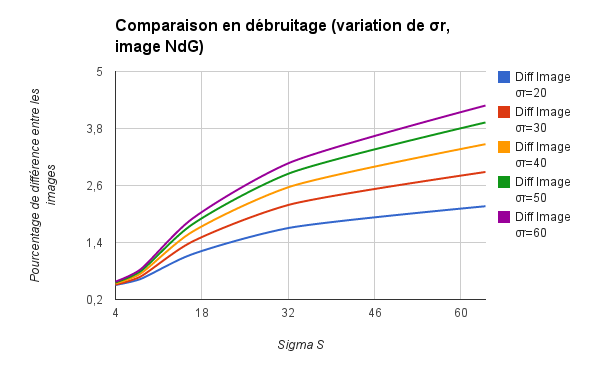
\includegraphics[scale=0.5]{images/debruitageNdGSigmaRDiffImage.png}

\end{frame}

\begin{frame}\frametitle{Résultat}

	\centering
	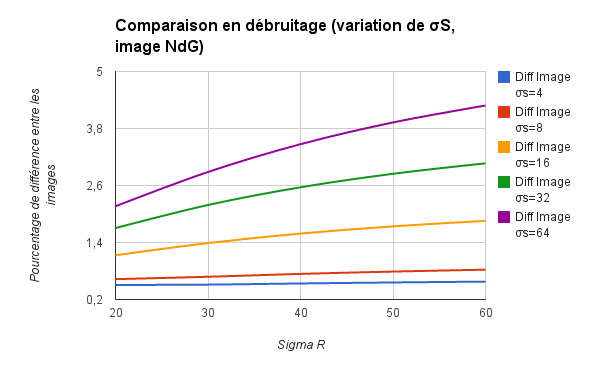
\includegraphics[scale=0.5]{images/debruitageNdGSigmaSDiffImage.png}
\end{frame}


\section{Pyramide}
\subsection{Décomposition}
\begin{frame}\frametitle{Définitions (1 sur 2)}
	\begin{block}{Définition}
		\begin{itemize}
			\item $u$ : couche de base
			\item $v$ : couche de détails
		\end{itemize}
	\end{block}
	\centering
	
\includegraphics[scale=0.3]{images/decompo.png}
\end{frame}

\begin{frame}\frametitle{Définitions (2 sur 2)}
	\begin{block}{Formulation}
		\begin{itemize}
			\item Décomposition à $(k+1)$ niveaux
			\item $u^1$, $\ldots$, $u^k$ : les versions filtrés de g
			\item $u^k = b$ : dernière couche de base
			\item $u^0 = g$ 
			\item $v^i = u^{i-1} - u^i$ : couche de détail 
		\end{itemize}
	\end{block}
\pause
	\begin{block}{Reconstruction}
		\begin{itemize}
			\item $g = b + \sum_{i=1}^{k}v^i$
		\end{itemize}
	\end{block}
	
\end{frame}

\begin{frame} \frametitle{Exemple}
\begin{figure}
	\center
	\subfloat[Image originale]{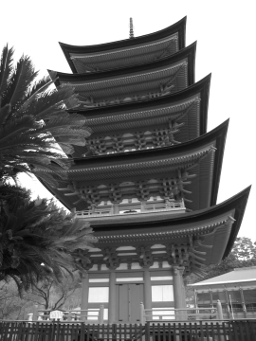
\includegraphics[scale=0.4]{images/IM088.png}}
	~
	\subfloat[Couche de base]{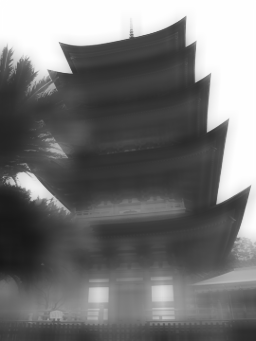
\includegraphics[scale=0.4]{images/pyramide_methode1_base_it_1_Ss_36_Sr_100_IM088.png}}
	~	
	\subfloat[Couche de détails]{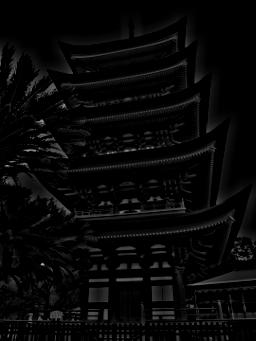
\includegraphics[scale=0.4]{images/pyramide_methode1_detail_it_1_Ss_36_Sr_100_IM088.png}}
\end{figure}
\end{frame}

\subsection{Méthodes}
\begin{frame}\frametitle{Méthodes}
	\begin{block}{Méthode 1}
		\begin{itemize}
			\item Filtrage toujours sur l'image originale
			\item Variation uniquement de $\sigma_s$ et $\sigma_r$
			\item $u^{i+1} = BF[g]$
		\end{itemize}
	\end{block}
\pause	
	\begin{block}{Méthode 2}
		\begin{itemize}
			\item Filtrage à partir de la dernière image obtenue
			\item $u^{i+1} = BF[u^i]$
		\end{itemize}
	\end{block}

\end{frame}

\subsection{Stratégies}
\begin{frame}\frametitle{Stratégies}
	\begin{block}{Stratégie 1}
		\begin{itemize}
			\item Variation de $\sigma_s$ et $\sigma_r$
		\end{itemize}
	\end{block}
\pause
	\begin{block}{Stratégie 2}
		\begin{itemize}
			\item Utilisation de la méthode 2
			\item Variation uniquement de $\sigma_r$
		\end{itemize}
	\end{block}
\end{frame}

\begin{frame}\frametitle{Exemple}
\begin{figure}
	\begin{center} 
		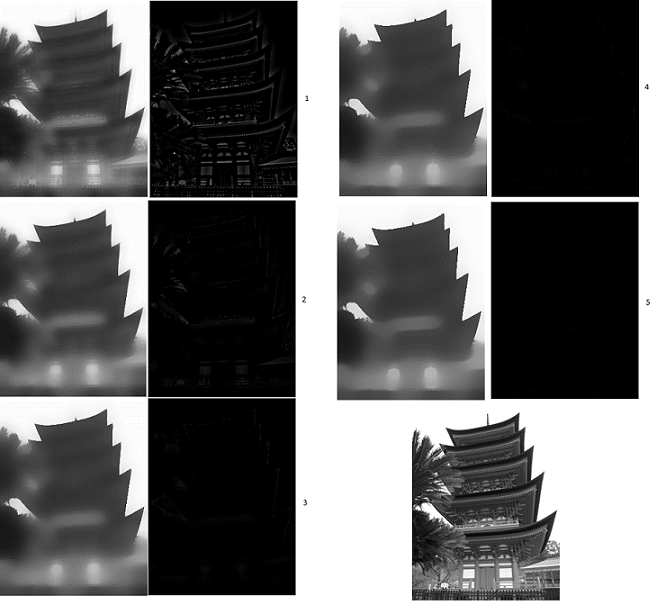
\includegraphics[scale=0.4]{images/pyramide2_rdiv2__36_100_IM088.png} 
	\end{center} 
	\caption{Décomposition pyramidale (méthode 2 et stratégie 2 - $\sigma_r$ divisé par 2), paramètre de départ $\sigma_s$=36 et $\sigma_r$=100}
\end{figure}
\end{frame}

\section{Manipulation}
\subsection{Définition}
\begin{frame}\frametitle{Définition}
	\begin{block}{Formulation}
		\begin{itemize}
			\item Ajout de paramètres : $\alpha$ et $\beta$
			\item $g = \alpha*b + \sum^{k}_{i=1}\beta*(i+1)*v^{i}$
		\end{itemize}
	\end{block}
\pause
	\begin{block}{Niveau de détails}
		\begin{itemize}
			\item Réhaussement : $\alpha < \beta$
			\item Atténuation : $\alpha > \beta$
		\end{itemize}
	\end{block}
	
\end{frame}

\subsection{Exemples}
\begin{frame}\frametitle{Réhaussement}
	\begin{figure}[H]
        \centering
        \subfloat[Méthode 1]{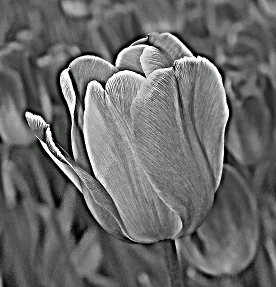
\includegraphics[scale=0.3]{images/flower1_08_3.png}}
        ~
        \subfloat[Méthode 2]{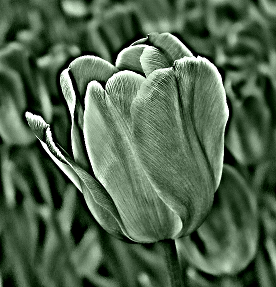
\includegraphics[scale=0.3]{images/flower2_08_3.png}}
        ~
        \subfloat[Image originale]{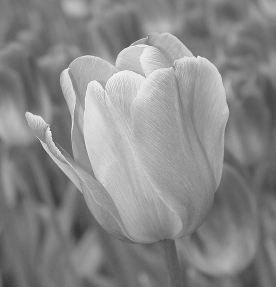
\includegraphics[scale=0.3]{images/flower2.png}}
        \caption{Réhaussement des détails avec $\alpha$=0.8 et $\beta$=3 (Stratégie 2)}
\end{figure}
\end{frame}

\begin{frame}\frametitle{Atténuation}

\begin{figure}
        \centering
        \subfloat[Méthode 1 et 2]{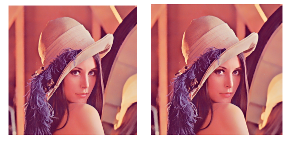
\includegraphics[scale=0.75]{images/lena_1_05.png}}
		~
        \subfloat[Image originale]{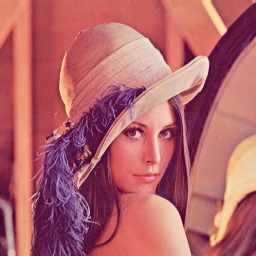
\includegraphics[scale=0.4]{images/lena.jpg}}
        \caption{Atténuation des détails avec $\alpha$=1 et $\beta$=0.5}
\end{figure}

\end{frame}

\section{Interface}
\subsection{Cas d'utilisation}
\begin{frame}\frametitle{Cas d'utilisation}
	\center
	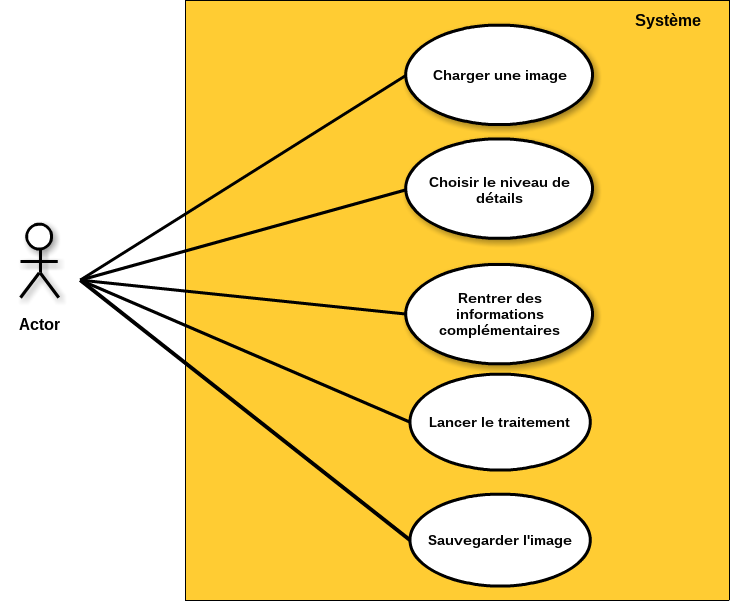
\includegraphics[scale=0.3]{images/UseCase.png}
\end{frame}

\subsection{Structure}
\begin{frame}\frametitle{Structure}
	\begin{block}{}
		\begin{itemize}
			\item C++ / Qt
			\item Modèle MVC (Modèle Vue Contrôleur)
			\item Librairie CImg
		\end{itemize}
	\end{block}
\end{frame}

\begin{frame}\frametitle{Interface}
	\center
	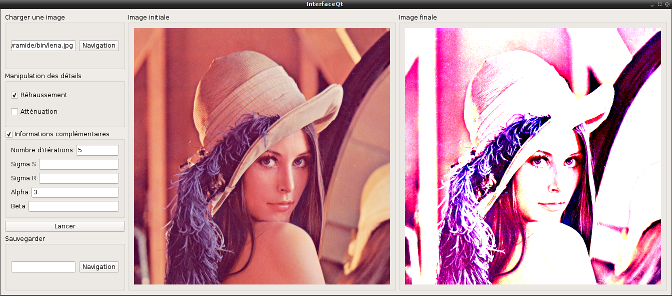
\includegraphics[scale=0.4]{images/screenIHMLaunch.png}
\end{frame}

\section{Accélération}
\begin{frame}\frametitle{Rappels}
	\begin{block}{Filtre Bilatéral}
		\begin{itemize}
			\item non-linéaire : chaque pixel est remplacé par un poids de ses voisins
			\item et non-itératif : le résultat est obtenu en un seul passage
			\item $I_p^{bf} = \frac{1}{W_p^{bf}}\sum_{q\in S} G_{\sigma_s}(\parallel p- q \parallel)G_{\sigma_r}(\mid I_p - I_q \mid) I_q$
			\item $W_p^{bf} = \sum_{q\in S} G_{\sigma_s}(\parallel p- q \parallel)G_{\sigma_r}(\mid I_p - I_q \mid)$
		\end{itemize}
	\end{block}
\pause
	\begin{block}{Non-linéarité}
		\begin{itemize}
			\item Division par $W_p^{bf}$
			\item Dépendance entre l'intensité des pixels par $G_{\sigma_r}(\mid I_p -I_q\mid)$
		\end{itemize}
	\end{block}
\end{frame}

\subsection{Intensité homogène}
\begin{frame}\frametitle{Intensité homogène}
	\begin{block}{Suppression de la division}
		\begin{itemize}
			\item $\binom{W_p^{bf} I_p^{bf}}{W_p^{bf}} = \sum_{q\in S} G_{\sigma_s}(\parallel p- q \parallel)G_{\sigma_r}(\mid I_p - I_q \mid) \binom{I_q}{1}$
			\item $\binom{W_p^{bf} I_p^{bf}}{W_p^{bf}} = \sum_{q\in S} G_{\sigma_s}(\parallel p- q \parallel)G_{\sigma_r}(\mid I_p - I_q \mid) \binom{W_q I_q}{W_q}$
			
		\end{itemize}
	\end{block}
\end{frame}

\subsection{Convolution}
\begin{frame}\frametitle{Convolution (1 sur 2)}
	\begin{block}{Symbole de Kronecker}
		\begin{itemize}
			\item $\delta(\zeta)$ (1 si $\zeta = 0$, 0 sinon)
			\item $[\delta(\zeta-I_q)=1] \leftrightarrow [\zeta = I_q]$
		\end{itemize}
	\end{block}
	$\binom{W_p^{bf} I_p^{bf}}{W_p^{bf}} = \sum_{q\in S}\sum_{\zeta\in R} G_{\sigma_s}(\parallel p- q \parallel)G_{\sigma_r}(\mid I_p - \zeta \mid)\delta(\zeta-I_q) \binom{W_q I_q}{W_q}$
	
\end{frame}

\begin{frame}\frametitle{Convolution (2 sur 2)}
	\begin{block}{Nouvelles fonctions}
		\begin{itemize}
			\item $g_{\sigma_s ,\sigma_r} : (x\in S, \zeta \in R) \mapsto G_{\sigma_s}[\parallel x \parallel)G_{\sigma_r}(\mid \zeta \mid)$
			\item $i : (x\in S, \zeta \in R) \mapsto I_x$ 
			\item $w : (x\in S, \zeta \in R) \mapsto \delta(\zeta - I_x)W_x$
		\end{itemize}
	\end{block}		
\pause
	\begin{block}{Conclusion}
		\begin{itemize}
		\item $\binom{W_p^{bf} I_p^{bf}}{W_p^{bf}} = \sum_{(q,\zeta)\in SxR} g_{\sigma_s ,\sigma_r}(p-q, I_p -\zeta)\binom{w(q,\zeta)i(q,\zeta)}{w(q,\zeta)}$
		\item $\binom{W_p^{bf} I_p^{bf}}{W_p^{bf}} = \left[ g_{\sigma_s ,\sigma_r} \otimes \binom{wi}{w}\right] (p,I_p)$
		\item linéaire : $(w^{bf}i^{bf}, w^{bf}) = g_{\sigma_s ,\sigma_r} \otimes (wi,w)$
		\item non-linéaire : $I_p^{bf} = \frac{w^{bf}(p,I_p)i^{bf}(p,I_p)}{w^{bf}(p,I_p)}$
		\end{itemize}
	
	\end{block}
	
\end{frame}

\subsection{Processus}
\begin{frame}\frametitle{Processus (Signal 1D)}
	\begin{columns}[t]
  		\begin{column}{5cm}
  			\begin{block}{}
    			\begin{itemize}
    				\item Données de bases
    				\item Représentation par une fonction à deux dimensions $(wi,w)$ 	
    				\item Convolution gaussienne $(w^{bf}i^{bf},w^{bf})$ 
    				\item Division
    				\item  Extraction par échantillonnage de la valeur à la position des données de bases
    			\end{itemize}
 			 \end{block} 
 		 \end{column}
  
		\begin{column}{6cm}
			\center
			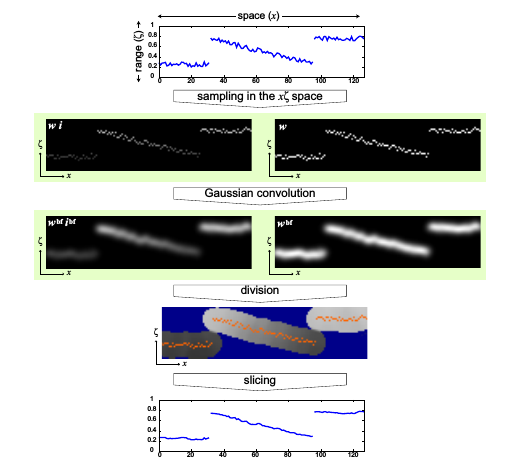
\includegraphics[scale=0.3]{images/processConvo.png}  
  		\end{column}
 	\end{columns} 	
	
	
\end{frame}

\subsection{Benchmark}
\begin{frame}\frametitle{Benchmark}

\begin{figure}
	\center
	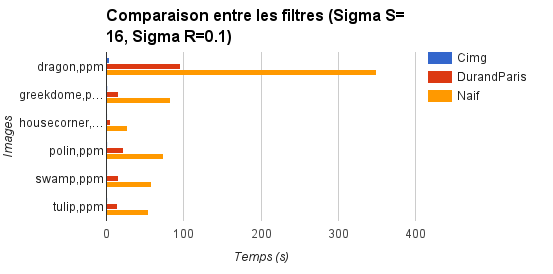
\includegraphics[scale=0.4]{images/benchmarkFiltreS16R01.png}
	\caption{$\sigma_s=16$ et $\sigma_r=0.1$}
\end{figure}	
\end{frame}

\section{Conclusion}
\subsection*{Planning}
\begin{frame}\frametitle{Planning}
	\begin{figure}
	\center
	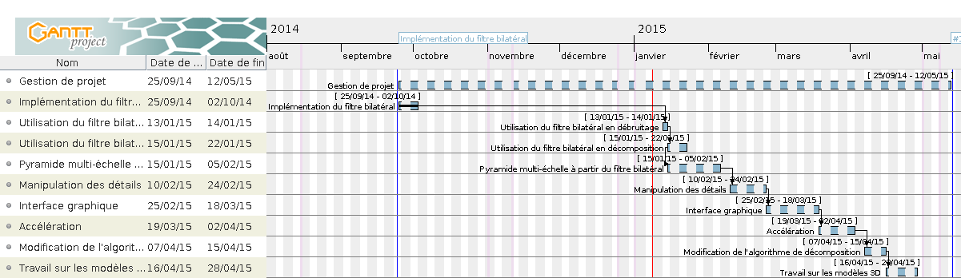
\includegraphics[width=320px]{images/Gantt.png}
\end{figure}
\end{frame}

\subsection*{Gestion de projet}
\begin{frame}\frametitle{Gestion de projet}
	\begin{block}{}
		\begin{itemize}
			\item Git
			\item Cycle en V
			\item Prise de contact régulière 
		\end{itemize}
	\end{block}

\end{frame}

\subsection*{Bilan}
\begin{frame}\frametitle{Bilan}
	\begin{block}{Travail fini}
		\begin{itemize}
			\item application avec filtre na\"if
			\item application avec filtre optimisé
		\end{itemize}
	\end{block}
	\begin{block}{Améliorations}
		\begin{itemize}
			\item Objet 3D
			\item Niveaux de manipulations supplémentaires
			\item Nouveaux paramètres de base
			\item Reconstruction avec des gradients
		\end{itemize}
	\end{block}
\end{frame}



\end{document}
